
\documentclass[letterpaper,12pt]{article}

\usepackage{hyperref}
\usepackage{graphicx}

\author{Jared Jensen}
\title{Behavioral Cloning}
\begin{document}
	\maketitle{}

	This is the first project where, after reading the instructions, I felt like I had no idea what I was going to do to complete the project but I knew I had the resources to ultimately complete the project. That was incredibly refreshing and the fact that everything was doing and everything I was trying was self-motivated made it that much more addicting. There were so many times where I had thought "Well, this might be the best I can do", tried it, and then that didn't work out, so I had to find a solution around it. It was mentally exhausting, cost me a lot of money in Amazon EC2 server time, and took around 8 hours a day for the better part of a week to complete, but I'm really happy with the finished product, and seeing the car drive around the track without crashing the first time was so rewarding, as it continues to be every time that I watch it.

	There were many setbacks. I initially made the entire model in TensorFlow, but then I had problems saving the model to a Keras-compatible .h5 file. I tried implementing a network that took in three images (left,right,center) simultaneously, then discovered that the program we're testing on only sends back the center image. I had a big problem where my network was running into a local minimum about 9/10 times, but would turn out a good model that 1/10 times. I had to experiment with that quite a bit to try and get over that hump more consistently.

	Here's what my final model looked like:

	\subsection*{Image Preprocessing}
	\begin{center}


		Collect one big list of center images, left images, and right  images (in that order)\\
		$\Downarrow$\\
		Turn each image into an array and rescale to 200x66\\
		$\Downarrow$\\
		Make a flipped version of the image, add flipped and nonflipped image to dictionary log\_data\\
		$\Downarrow$\\
		Add steering angle (and reversed steering angle), throttle, braking, and speed to log data, then repeat the big list two more times (for left and right images)\\
		$\Downarrow$\\
		Remove all images in a certain range of steering angles according to input (I didn't actually end up using this because I found the car drives smoother when it had a lot of straight examples)\\
		$\Downarrow$\\
		Rescale all images down to 1/255 values, so the data lies between 1 and -1.\\
		$\Downarrow$\\
		Feed into image generator which would shift image up or down to a value of 1/5 of its width or height, and replace unused space with black\\

	\end{center}

	\subsection*{Model}
	I used NVIDIA's model from \href{http://images.nvidia.com/content/tegra/automotive/images/2016/solutions/pdf/end-to-end-dl-using-px.pdf}{here} almost verbatim. I just added a couple of dropout layers to prevent overfitting. Here's what it looks like.
	\begin{center}

		Convolution 1. Input: (?, 66, 200, 3) Output: (?, 31, 98, 24) Kernel: 5x5 Stride: 2x2 Activation: Relu\\
		$\Downarrow$\\
		Convolution 2. Input: (?, 31, 98, 24) Output: (?, 14, 47, 36) Kernel: 5x5 Stride: 2x2 Activation: Relu\\
		$\Downarrow$\\
		Convolution 3. Input: (?, 14, 47, 36) Output: (?, 5, 22, 48) Kernel: 5x5 Stride: 2x2 Activation: Relu\\
		$\Downarrow$\\
		Convolution 4. Input: (?, 5, 22, 48) Output: (?, 3, 20, 64) Kernel: 3x3 Stride: 1x1 Activation: Relu\\
		$\Downarrow$\\
		Convolution 5. Input: (?, 3, 20, 64) Output: (?, 1, 18, 64) Kernel: 3x3 Stride: 1x1 Activation: Relu\\
		$\Downarrow$\\
		Dropout 1. .5 Chance\\
		$\Downarrow$\\
		Flatten. Input: (?, 1, 18, 64) Output: (?, 1152)\\
		$\Downarrow$\\
		Fully Connected 1. Input: (?, 1152) Output: (?, 100) Activation: Relu\\
		$\Downarrow$\\
		Fully connected 2. Input: (?, 100) Output: (?, 50) Activation: Relu\\
		$\Downarrow$\\
		Fully connected 3. Input: (?, 50) Output: (?, 10) Activation: Relu\\
		$\Downarrow$\\
		Dropout 2. .5 Chance\\
		$\Downarrow$\\
		Output layer: 1 output

	\end{center}

\subsection*{Training}
I used a Nadam optimizer because it has all of the stochastic benefits of an Adam optimizer with the momentum feature to help get over local minima. I then trained in two stages.
\begin{enumerate}
\item 20 epochs with a learning rate of .001 on a full two laps around the course. This built a solid base and got my car running on the straights well, but it wasn't turning enough for some corners.

\item 10 epochs with a learning rate of .001 on one lap of just the twisty part of the course. I did this because the car wasn't turning enough and would go off the road on some of the twisty parts.
\end{enumerate}
I found this solution to be a good combination of smooth driving (which is really important when your car is going fast) and hard cornering. I set the throttle to 100\% the whole time, and the car goes around the track 9/10 times without crashing. The car goes around the track with an even higher success rate when throttle is set to something more manageable, like 20\% (which ends up getting up to about 66\% speed)

Here are some examples of the dataset used to train the network:

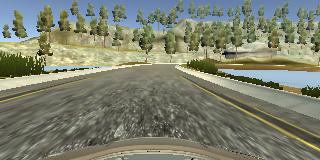
\includegraphics{sample_images/center_2016_12_01_13_32_58_012.jpg}\\
Steering angle: -0.1167233

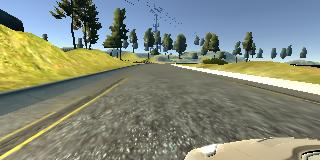
\includegraphics{sample_images/left_2016_12_01_13_38_11_408.jpg}\\
Steering angle: 0

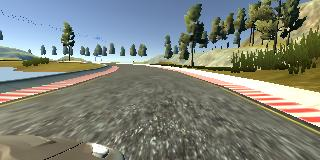
\includegraphics{sample_images/right_2016_12_01_13_45_55_778.jpg}\\
Steering angle: 0.3201102

\end{document}
